\section{Unsupervised keypoint learning}

In order to build a map it is useful to extract features, or landmarks, from images. Every feature should have a unique descriptor which can be used to identify the features in the map in order to expand the map and localize the camera. How to build a map and localize in it is out of scope for this thesis. This section will describe an unsupervised learning method to extract features from images that would be usable in a full SFML pipeline.

The method evaluated in this thesis is based on the Unsuperpoint paper \cite{unsuperpoint} from 2019. The network architecture is illustrated in Figure \ref{fig:unsuperpoint}. The input image is fed into a shared backbone. The features from the backbone are then split into three different encoders that estimate the score, position and a descriptor for each feature. The network will estimate a feature in every $8\times 8$ patch of the image, but only the top $N$ features sorted by score are used in the evaluation.

\begin{figure}[H]
	\centering
	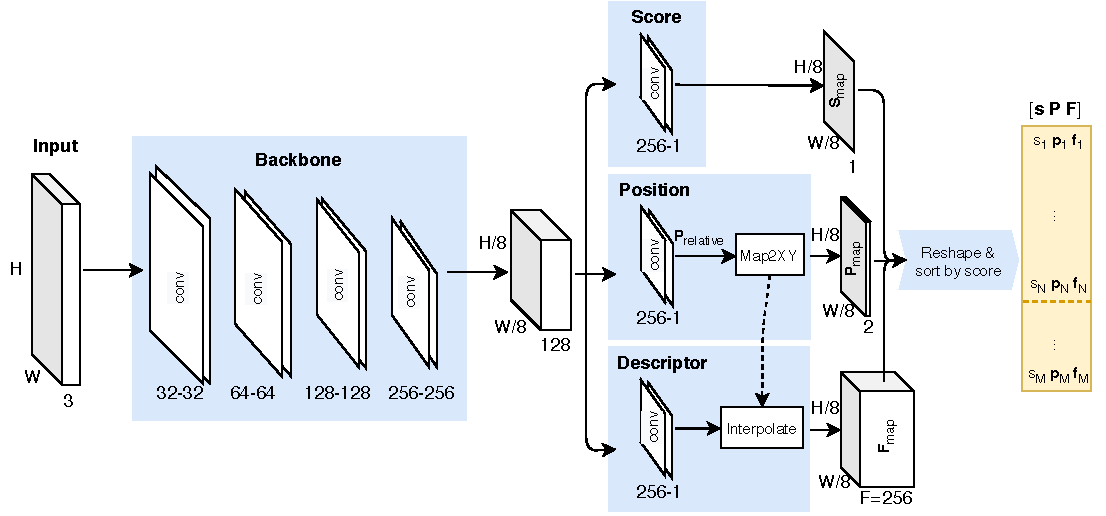
\includegraphics[width=1.0\textwidth]{unsuperpoint}
	\caption{The network has a common backbone and then splits into separate score, position and descriptor encoders. The output is reshaped and sorted by descending score.}
	\label{fig:unsuperpoint}
\end{figure}

The network is trained in a siamese twin setup, where two duplicate networks that share weights are fed different inputs and the loss is formulated by comparing the output scores, positions and descriptors.

\begin{figure}[H]
	\centering
	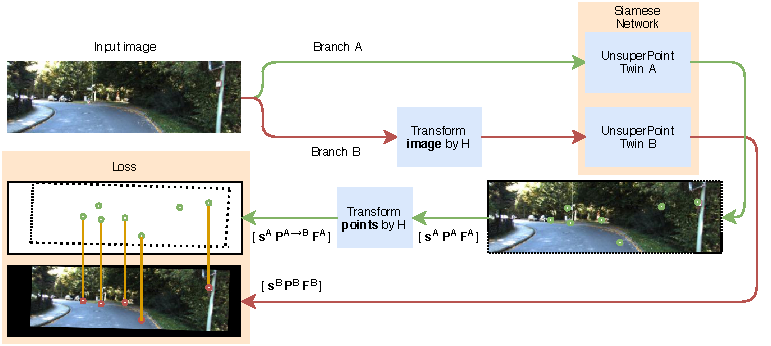
\includegraphics[width=1.0\textwidth]{unsuperpointloss}
	\caption{}
	\label{fig:unsuperpointloss}
\end{figure}

The backbone consists of four groups of convolution, batch norm, ReLu and max pooling operations.

\subsection{Score encoder}

The score encoder 

Brute force matching using PyTorch instead of OpenCV because we want to use the result as input to the next consensus step.